\documentclass[aspectratio=169,10pt,t]{beamer}
\usepackage{issa}  % place issa.sty in the same folder
\definecolor{AccentCol}{HTML}{1B7A5E}
\renewcommand{\lecnum}{7}
\begin{document}
\titleslide{7}{Reinforcement Learning Part 2:\\Policy Gradient Methods}{REINFORCE \textbullet\ baselines \textbullet\ actor--critic \textbullet\ A2C/A3C \textbullet\ PPO \textbullet\ continuous control \textbullet\ SAC\\Case study: 4-drone autonomous swarm, continuous waypoint control, 6-DoF flight dynamics, PPO vs SAC}

\sect{1. Why Policy Gradients}
\begin{frame}{When DQN Is Not Enough --- Q-Learning Needs a Discrete Action Space}
\begin{columns}[T]
\column{0.50\textwidth}
\begin{cbox}[ISSAred]{Value-based (DQN) limitations}\scriptsize Policy $\pi(s)=\arg\max_aQ(s,a;\theta)$ works when the action space is DISCRETE and SMALL ($|A|=7$ in the wargame). It breaks down for: \textbf{continuous} actions --- drone thrust $\in[-100,+100]^3$ N has infinitely many values, so the argmax becomes an optimisation inside every step; \textbf{huge discrete} spaces --- 50,000-token vocabularies mean 50K Q-values per pass; and exploration is bolted on ($\varepsilon$-greedy).\end{cbox}
\figc{2.0cm}{\begin{tikzpicture}\draw[->](0,0)--(5.2,0)node[right,font=\tiny]{thrust};\draw[AccentCol,thick,domain=0:5,samples=50]plot(\x,{1.2*exp(-(\x-3.1)^2/0.5)});\draw[dashed](3.1,0)--(3.1,1.25);\node[font=\tiny,anchor=south]at(3.1,1.25){$\mu_\theta(s)$};\draw[<->,ISSAred](2.4,0.45)--(3.8,0.45)node[midway,below,font=\tiny]{$\sigma_\theta(s)$};\node[lab]at(2.6,-0.35){the policy outputs a distribution; sample, don't argmax};\end{tikzpicture}}
\column{0.48\textwidth}
\begin{fbx}{Policy gradient theorem}\[\nabla_\theta J(\theta)=\mathbb{E}_{\tau\sim\pi_\theta}\Big[\sum_t\nabla_\theta\log\pi_\theta(a_t|s_t)\,G_t\Big]\]\[G_t=\sum_{k\ge t}\gamma^{k-t}r_{k+1}\]\end{fbx}
\begin{tl}\item Parameterise the POLICY $\pi_\theta(a|s)$ directly instead of learning values as an intermediary\item ``Make actions that led to high return MORE probable by moving $\theta$ along the gradient of their log-probability''\item Continuous actions become trivial: $\pi_\theta(a|s)=\mathcal{N}(\mu_\theta(s),\sigma_\theta(s)^2)$\item A stochastic policy gives \textbf{natural exploration}\end{tl}
\end{columns}
\end{frame}

\begin{frame}{Policy Gradient Intuition --- Shifting Probability Toward Good Actions}
\begin{columns}[T]
\column{0.52\textwidth}
\figc{3.3cm}{\begin{tikzpicture}\begin{axis}[width=7.2cm,height=4.0cm,xlabel={action (e.g.\ heading change, degrees)},ylabel={$\pi_\theta(a|s)$},domain=-30:30,samples=80,ytick=\empty,legend pos=north west]
\addplot[ISSAgrey,thick,dashed]{exp(-(x+5)^2/(2*64))};\addlegendentry{before update}
\addplot[AccentCol,thick]{exp(-(x-4)^2/(2*36))};\addlegendentry{after update}
\draw[ISSAgrn,thick,->](axis cs:-5,1.05)--(axis cs:4,1.05);\node[font=\tiny,ISSAgrn,anchor=south]at(axis cs:0,1.06){high-return actions pull the mean};
\fill[ISSAgrn](axis cs:6,0.02)circle(2pt);\node[font=\tiny,ISSAgrn,anchor=south]at(axis cs:9,0.08){$G$ high};\fill[ISSAred](axis cs:-15,0.02)circle(2pt);\node[font=\tiny,ISSAred,anchor=south]at(axis cs:-17,0.08){$G$ low};
\end{axis}\end{tikzpicture}}
\column{0.46\textwidth}
\begin{cbox}{Why the log-probability?}\scriptsize $\nabla_\theta\log\pi_\theta(a|s)=\nabla_\theta\pi_\theta(a|s)/\pi_\theta(a|s)$ --- the \textbf{score function}. It tells us how to change $\theta$ to make action $a$ more likely; dividing by $\pi$ avoids over-reinforcing actions that are already frequent.\end{cbox}
\begin{ibox}\scriptsize\textbf{Analogy:} after-action reviews. Tactics used in successful sorties get trained more often; tactics used in failed ones are de-emphasised --- without anyone writing down the ``correct'' manoeuvre for each situation.\end{ibox}
\begin{wbox}\scriptsize But a whole sortie's outcome is a noisy verdict on any single decision --- the variance problem (three slides ahead).\end{wbox}
\end{columns}
\end{frame}

\sect{2. REINFORCE}
\begin{frame}{REINFORCE (Williams 1992) --- Complete Episodes, Then Update}
\begin{columns}[T]
\column{0.50\textwidth}
\begin{cbox}{Algorithm}\scriptsize Initialise $\theta$ randomly. For each episode: \textbf{1.} run $\pi_\theta$ to generate $\tau=(s_0,a_0,r_1,\ldots,s_T)$; \textbf{2.} for each $t$ compute $G_t=\sum_{k=t}^{T-1}\gamma^{k-t}r_{k+1}$; \textbf{3.} update $\theta\leftarrow\theta+\alpha\,G_t\nabla_\theta\log\pi_\theta(a_t|s_t)$. Batch form: $\nabla J\approx\frac1T\sum_tG_t\nabla_\theta\log\pi_\theta(a_t|s_t)$.\end{cbox}
\begin{fbx}{REINFORCE update}\[\theta\leftarrow\theta+\alpha\,G_t\,\nabla_\theta\log\pi_\theta(a_t|s_t)\]\end{fbx}
\column{0.48\textwidth}
\begin{cbox}[ISSAgrn]{Strengths}\scriptsize $\checkmark$ unbiased gradient estimate (Monte Carlo) $\checkmark$ works for discrete AND continuous actions $\checkmark$ simple to implement.\end{cbox}
\begin{cbox}[ISSAred]{Weaknesses}\scriptsize $\times$ HIGH VARIANCE: $G_t$ sums a whole noisy trajectory $\times$ needs complete episodes before any update $\times$ sample-inefficient: each episode used once $\times$ can forget early experience.\end{cbox}
\figc{1.5cm}{\begin{tikzpicture}\foreach \i in {0,...,5}{\node[circle,draw=AccentCol,fill=AccentCol!15,inner sep=1.5pt,font=\tiny](s\i)at(\i*1.1,0){$s_\i$};}\foreach \i/\jj in {0/1,1/2,2/3,3/4,4/5}{\draw[arr](s\i)--(s\jj);}\draw[ISSAred,thick,decorate,decoration={brace,amplitude=4pt,mirror}](0,-0.35)--(5.5,-0.35)node[midway,below=4pt,font=\tiny]{wait for the whole episode, then compute every $G_t$};\end{tikzpicture}}
\end{columns}
\end{frame}

\begin{frame}{Drone Swarm Case Study --- Setup and the REINFORCE Baseline}
\begin{columns}[T]
\column{0.50\textwidth}
\figc{2.9cm}{\begin{tikzpicture}[x=0.6cm,y=0.6cm]
\draw[ISSAgrey,fill=ISSAgrn!5](0,0)rectangle(9,5);
\foreach \x/\y in {2.2/3.2,5.0/1.4,6.8/3.6}{\fill[ISSAred!25,draw=ISSAred](\x,\y)circle(0.7);}\node[font=\tiny,ISSAred]at(5.0,1.4){no-fly};
\foreach \i/\x/\y in {1/1.2/1.0,2/3.6/1.6,3/4.2/3.8,4/6.0/2.6,5/8.2/4.4}{\node[circle,draw=AccentCol,fill=white,inner sep=1pt,font=\tiny]at(\x,\y){\i};}
\draw[AccentCol,dashed](1.2,1.0)--(3.6,1.6)--(4.2,3.8)--(6.0,2.6)--(8.2,4.4);
\foreach \x/\y in {0.4/0.4,0.8/0.3,0.5/0.8,0.9/0.7}{\node[regular polygon,regular polygon sides=3,fill=ISSAnavy,inner sep=1.2pt]at(\x,\y){};}
\node[lab,anchor=west]at(0.1,5.3){4 drones $\to$ 5 waypoints in sequence, avoiding 3 no-fly zones};
\end{tikzpicture}}
\begin{cbox}[ISSAnavy]{State and action}\scriptsize Per drone 18 features (position, velocity, fuel, 8 obstacle clearances, waypoint relative position) $\times$ 4 drones = 72 + swarm centroid (3) + formation metrics (5) = \textbf{80}. Action: continuous thrust $[F_x,F_y,F_z]$ per drone = \textbf{12-dim}.\end{cbox}
\column{0.48\textwidth}
\begin{cbox}{REINFORCE (no baseline)}\scriptsize Network $80\to256\to256\to\mu(12)+\log\sigma(12)$; 10,000 episodes, batch 1.\end{cbox}
\figc{2.3cm}{\bars{100}{1.6}{2.1}{Waypoint success (\%)/61.4/AccentCol,Collision rate (\%)/8.4/ISSAred}}
\begin{wbox}\scriptsize Average return $142.8\pm\mathbf{84.6}$: very high variance $\Rightarrow$ unstable learning. 6,200 episodes to reach 50\% success.\end{wbox}
\end{columns}
\end{frame}

\sect{3. Baselines \& Advantage}
\begin{frame}{The Variance Problem --- A High Return Does Not Mean the Action Was Good}
\begin{columns}[T]
\column{0.52\textwidth}
\figc{2.9cm}{\begin{tikzpicture}
\node[ndR,text width=5.6cm,align=left](e1)at(0,0.9){\textbf{Episode 1:} drone A makes a turn 5$^\circ$ off optimal at $t=3$; the episode goes well for other reasons ($G_t=180$). $\Rightarrow$ the update \textbf{increases} the probability of the poor turn.};
\node[ndR,text width=5.6cm,align=left](e2)at(0,-0.75){\textbf{Episode 2:} the same drone makes a good turn; bad fuel luck ($G_t=40$). $\Rightarrow$ the update \textbf{decreases} the probability of the good turn.};
\end{tikzpicture}}
\begin{wbox}\scriptsize\textbf{Root cause:} $G_t$ mixes the quality of the specific action $a_t$ with all the luck and skill of the rest of the episode. We want credit only for the \emph{relative} value of $a_t$ against the alternatives.\end{wbox}
\column{0.46\textwidth}
\begin{fbx}{Baseline: unbiased variance reduction}\[\theta\leftarrow\theta+\alpha\,(G_t-b(s_t))\,\nabla_\theta\log\pi_\theta(a_t|s_t)\]\[\mathbb{E}\big[\nabla\log\pi\cdot b(s)\big]=b(s)\,\mathbb{E}[\nabla\log\pi]=0\]\end{fbx}
\begin{fbx}{Best baseline $\Rightarrow$ the advantage}\[b(s)=V^{\pi}(s),\qquad A(s,a)=Q(s,a)-V(s)\]\end{fbx}
\sm{$A>0$: better than average $\Rightarrow$ increase probability; $A<0$: worse $\Rightarrow$ decrease; $A=0$: no update. The baseline must not depend on $a$.}
\end{columns}
\end{frame}

\begin{frame}{Baselines in Practice --- Variance Halved With No Bias}
\begin{columns}[T]
\column{0.50\textwidth}
\figc{3.2cm}{\begin{tikzpicture}\begin{axis}[width=7.0cm,height=3.8cm,xlabel={training episode},ylabel={return},xmin=0,xmax=100,ymin=0,ymax=300,ticks=none,domain=0:100,samples=60,legend pos=north west]
\addplot[name path=a1,draw=none]{60+0.9*x+84};\addplot[name path=a2,draw=none]{60+0.9*x-84};\addplot[ISSAred!20]fill between[of=a1 and a2];\addlegendentry{REINFORCE $\pm$84.6}
\addplot[name path=b1,draw=none]{70+1.2*x+41};\addplot[name path=b2,draw=none]{70+1.2*x-41};\addplot[AccentCol!35]fill between[of=b1 and b2];\addlegendentry{+ baseline $\pm$41.2}
\addplot[ISSAred,thick]{60+0.9*x};\addplot[AccentCol,thick]{70+1.2*x};
\end{axis}\end{tikzpicture}}
\sm{Schematic learning curves; the band widths are the reported return standard deviations.}
\column{0.48\textwidth}
\figc{2.4cm}{\bars{100}{1.7}{2.1}{REINFORCE/61.4/ISSAred,REINFORCE + baseline $V_\phi(s)$/72.1/AccentCol}}
\sm{Waypoint success (\%): +10.7 points from the baseline alone.}
\begin{ibox}\scriptsize\textbf{Bias--variance trade-off:} REINFORCE is unbiased but high-variance; a $V(s)$ baseline cuts variance at NO bias. Actor--critic (next) cuts variance further by bootstrapping --- at the cost of some bias from the value estimate. PPO controls this trade-off carefully.\end{ibox}
\end{columns}
\end{frame}

\sect{4. Actor-Critic}
\begin{frame}{Actor--Critic --- Two Networks, One Learning Loop}
\begin{columns}[T]
\column{0.50\textwidth}
\figc{2.9cm}{\begin{tikzpicture}
\node[nd](s)at(0,0){state $s$};\node[ndA,minimum width=2.2cm,minimum height=0.9cm](ac)at(2.8,0.9){\textbf{ACTOR} $\pi_\theta(a|s)$\\\sm{$\mu(s)$, $\log\sigma(s)$}};\node[ndN,minimum width=2.2cm,minimum height=0.9cm](cr)at(2.8,-0.9){\textbf{CRITIC} $V_\phi(s)$\\\sm{scalar value}};\node[nd](env)at(5.6,0.9){environment};
\draw[arr](s)--(ac);\draw[arr](s)--(cr);\draw[arr](ac)--node[above,font=\tiny]{$a$}(env);\draw[arr](env.south)|-node[pos=0.3,right,font=\tiny]{$r$, $s'$}(cr.east);\draw[arr,ISSAred](cr.north)--node[right,font=\tiny,ISSAred]{$\hat A=r+\gamma V(s')-V(s)$}(ac.south);
\end{tikzpicture}}
\begin{fbx}{Losses}\[L_{\text{actor}}=-\mathbb{E}\big[\hat A(s,a)\log\pi_\theta(a|s)\big]\]\[L_{\text{critic}}=\mathbb{E}\big[(G_t-V_\phi(s))^{2}\big]\]\[L(\theta,\phi)=L_{\text{actor}}+c_1L_{\text{critic}}-c_2H(\pi_\theta)\]\end{fbx}
\column{0.48\textwidth}
\begin{tl}\item \textbf{Actor:} discrete $\to$ softmax over actions; continuous $\to$ Gaussian $\mu(s)$, $\log\sigma(s)$\item \textbf{Critic:} supervised regression of returns\item \textbf{TD advantage} $\hat A=r+\gamma V_\phi(s')-V_\phi(s)$: the one-step TD error --- much lower variance than Monte-Carlo $G_t$, slight bias from $V_\phi$ errors\item \textbf{Entropy bonus} $H(\pi_\theta)$ keeps the policy exploring\end{tl}
\begin{ibox}\scriptsize\textbf{Military analogy:} the actor is the platoon commander choosing moves; the critic is the staff officer estimating how good each situation is, so every move can be judged immediately instead of waiting for the battle's outcome.\end{ibox}
\end{columns}
\end{frame}

\begin{frame}{A2C and A3C --- Parallel Workers for Lower Variance}
\begin{columns}[T]
\column{0.50\textwidth}
\figc{2.6cm}{\begin{tikzpicture}
\node[ndN,minimum width=2.2cm,minimum height=0.8cm](m)at(2.4,1.5){master network $\theta$};
\foreach \i in {1,...,4}{\node[ndA,minimum width=1.0cm](w\i)at(\i*1.2-0.6,0){worker \i};\draw[arr,<->](w\i)--(m);}
\node[lab]at(2.4,-0.65){A2C: all workers update together (synchronous)};
\end{tikzpicture}}
\begin{cbox}[ISSAgrn]{A2C --- synchronous}\scriptsize $N$ parallel environment workers collect experience simultaneously; the master updates from ALL together: more diverse experience, better variance reduction ($N$ samples per update), no staleness. Drone case: $N=4$ (one per drone).\end{cbox}
\column{0.48\textwidth}
\begin{cbox}[ISSAamb]{A3C --- asynchronous (Mnih 2016)}\scriptsize Each worker reads $\theta$, runs episodes and pushes gradients on its own schedule. Very efficient on CPUs (no GPU needed); diverse exploration. Weakness: \textbf{stale gradients} (workers use an old $\theta$), unstable at high parallelism.\end{cbox}
\figc{2.2cm}{\bars{100}{1.5}{2.1}{REINFORCE + baseline/72.1/ISSAamb,A2C ($N=4$ workers)/83.2/AccentCol}}
\sm{Waypoint success (\%): +11.1 points; return $194.8\pm\mathbf{28.4}$ --- variance reduced again.}
\end{columns}
\end{frame}

\sect{5. PPO}
\begin{frame}{Proximal Policy Optimisation --- Why Updates Must Stay Close}
\begin{columns}[T]
\column{0.50\textwidth}
\begin{wbox}\scriptsize\textbf{Problem with vanilla policy gradient:} a large step can change the policy dramatically and performance can \textbf{collapse} (e.g.\ $\pi$ suddenly starts crashing all drones); recovery takes thousands of episodes.\end{wbox}
\begin{cbox}[ISSAnavy]{Trust-region idea (TRPO, 2015)}\scriptsize Maximise the objective subject to $\text{KL}(\pi_{\text{old}}\|\pi_{\text{new}})\le\delta$ --- a proven monotonic-improvement guarantee, but it needs second-order (natural-gradient/Hessian) computation: prohibitive for large networks.\end{cbox}
\begin{rbox}\scriptsize\textbf{PPO (Schulman 2017):} replace the KL constraint with a clipped objective --- first-order SGD/Adam only, 3--10$\times$ cheaper than TRPO with similar performance. Today's gold standard.\end{rbox}
\column{0.48\textwidth}
\figc{3.2cm}{\begin{tikzpicture}\begin{axis}[width=6.4cm,height=3.8cm,xlabel={policy change (step size)},ylabel={performance},xmin=0,xmax=10,ymin=0,ymax=10,ticks=none,domain=0:10,samples=60]
\addplot[AccentCol,thick]{6+2.5*sin(deg(x*0.6))-0.15*(x-3)^2*(x>6)};
\fill[ISSAgrn!20,opacity=0.6](axis cs:2,0)rectangle(axis cs:4.5,10);\node[font=\tiny,ISSAgrn,anchor=north]at(axis cs:3.25,9.8){trust region};
\draw[ISSAred,thick,->](axis cs:3,7.4)--(axis cs:8.8,3.5);\node[font=\tiny,ISSAred,anchor=west]at(axis cs:6.3,6.6){big step: collapse};
\fill[AccentCol](axis cs:3,7.4)circle(2pt);
\end{axis}\end{tikzpicture}}
\sm{Schematic: the gradient is only trustworthy near the current policy.}
\end{columns}
\end{frame}

\begin{frame}{PPO --- The Clipped Surrogate Objective}
\begin{columns}[T]
\column{0.50\textwidth}
\begin{fbx}{Ratio and clipped objective}\[r_t(\theta)=\frac{\pi_\theta(a_t|s_t)}{\pi_{\theta_{\text{old}}}(a_t|s_t)}\]\[L^{\text{CLIP}}=\mathbb{E}_t\Big[\min\big(r_t\hat A_t,\ \text{clip}(r_t,1-\varepsilon,1+\varepsilon)\hat A_t\big)\Big]\]\end{fbx}
\begin{tl}\item $r_t=1$: unchanged; $>1$: action more likely; $<1$: less likely; typical $\varepsilon=0.2$\item $\hat A>0$ (good action): gain saturates at $r=1.2$ --- at most 20\% more likely per update\item $\hat A<0$ (bad action): saturates at $r=0.8$ --- at most 20\% less likely\item No action's probability can move more than $\pm20\%$ per update $\Rightarrow$ no catastrophic collapse\end{tl}
\column{0.48\textwidth}
\figc{2.2cm}{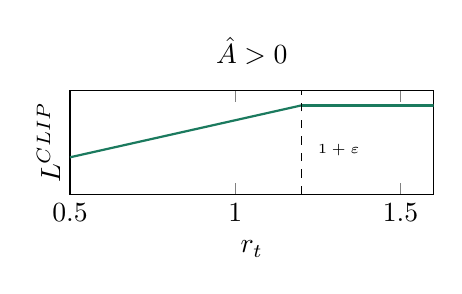
\begin{tikzpicture}\begin{axis}[width=6.2cm,height=2.9cm,xlabel={$r_t$},ylabel={$L^{\text{CLIP}}$},xmin=0.5,xmax=1.6,ymin=0,ymax=1.4,title={$\hat A>0$},ytick=\empty]
\addplot[AccentCol,thick,domain=0.5:1.2]{x};\addplot[AccentCol,thick,domain=1.2:1.6]{1.2};\draw[dashed](axis cs:1.2,0)--(axis cs:1.2,1.4);\node[font=\tiny,anchor=west]at(axis cs:1.22,0.6){$1+\varepsilon$};
\end{axis}\end{tikzpicture}}
\figc{2.2cm}{\begin{tikzpicture}\begin{axis}[width=6.2cm,height=2.9cm,xlabel={$r_t$},ylabel={$L^{\text{CLIP}}$},xmin=0.4,xmax=1.6,ymin=-1.6,ymax=0,title={$\hat A<0$},ytick=\empty]
\addplot[ISSAred,thick,domain=0.4:0.8]{-0.8};\addplot[ISSAred,thick,domain=0.8:1.6]{-x};\draw[dashed](axis cs:0.8,-1.6)--(axis cs:0.8,0);\node[font=\tiny,anchor=east]at(axis cs:0.78,-1.2){$1-\varepsilon$};
\end{axis}\end{tikzpicture}}
\sm{Flat regions = zero gradient: no incentive to push the policy further.}
\end{columns}
\end{frame}

\sect{6. Continuous Control}
\begin{frame}{Continuous Action Spaces --- the Gaussian Policy}
\begin{columns}[T]
\column{0.52\textwidth}
\begin{fbx}{Gaussian policy and reparameterisation}\[\pi_\theta(a|s)=\mathcal{N}\big(\mu_\theta(s),\text{diag}(\sigma_\theta(s)^2)\big)\]\[a=\mu_\theta(s)+\sigma_\theta(s)\odot\epsilon,\qquad\epsilon\sim\mathcal{N}(0,I)\]\[\log\pi_\theta(a|s)=-\tfrac12\sum_i\Big[\tfrac{(a_i-\mu_i)^2}{\sigma_i^2}+\log\sigma_i^2+\log2\pi\Big]\]\end{fbx}
\begin{tl}\item The network outputs $\mu_\theta(s)$ (nominal action) and $\log\sigma_\theta(s)$ (learned exploration; more stable than $\sigma$)\item Reparameterisation lets gradients flow through the sample; the log-probability is the term differentiated in the policy gradient\end{tl}
\column{0.46\textwidth}
\figc{2.6cm}{\begin{tikzpicture}\begin{axis}[width=6.4cm,height=3.2cm,xlabel={thrust command},domain=-4:4,samples=80,ytick=\empty,legend pos=north west]
\addplot[ISSAblue,thick]{exp(-x^2/(2*2.2))/1.2};\addlegendentry{free airspace: high $\sigma$}
\addplot[ISSAred,thick]{exp(-(x-1)^2/(2*0.12))};\addlegendentry{near obstacle: low $\sigma$}
\end{axis}\end{tikzpicture}}
\begin{rbox}\scriptsize\textbf{Bounded, state-dependent exploration:} high $\sigma$ in open high-altitude airspace (explore!), low $\sigma$ near obstacles (precise, focused actions). $\sigma$ is learned from the reward signal automatically.\end{rbox}
\end{columns}
\end{frame}

\begin{frame}{6-DoF Flight Dynamics --- What the Drone Policy Controls}
\begin{columns}[T]
\column{0.48\textwidth}
\figc{2.8cm}{\begin{tikzpicture}
\draw[fill=ISSAgrey!30](-0.5,-0.15)rectangle(0.5,0.15);\foreach \x/\y in {-1.0/0.35,1.0/0.35,-1.0/-0.35,1.0/-0.35}{\draw[ISSAnavy](\x,\y)ellipse(0.38 and 0.1);\draw(\x,\y)--(0,0);}
\draw[-{Stealth},ISSAred,thick](0,0)--(1.9,0)node[right,font=\tiny]{$x$ (roll $\phi$)};\draw[-{Stealth},ISSAgrn,thick](0,0)--(-1.1,-1.0)node[below,font=\tiny]{$y$ (pitch $\theta$)};\draw[-{Stealth},ISSAblue,thick](0,0)--(0,1.5)node[above,font=\tiny]{$z$ (yaw $\psi$)};
\draw[-{Stealth},AccentCol,line width=1.4pt](0.2,0.2)--(1.0,1.2)node[right,font=\tiny]{thrust $F$};
\end{tikzpicture}}
\begin{cbox}[ISSAnavy]{Six degrees of freedom}\scriptsize 3 translational ($x,y,z$) + 3 rotational (roll, pitch, yaw).\end{cbox}
\column{0.50\textwidth}
\begin{cbox}{State per drone (18) and action (3)}\scriptsize Position $[x,y,z]$; velocity $[v_x,v_y,v_z]$; orientation [roll, pitch, yaw]; angular rate $[p,q,r]$; fuel $F\in[0,1]$; waypoint offset $[\Delta x,\Delta y,\Delta z]$ = 16, + 2 safety flags = 18. Action: thrust $[F_x,F_y,F_z]$ (N); rotor-speed differential for yaw, simplified to 3-D.\end{cbox}
\begin{fbx}{Simplified Euler dynamics ($m=1.2$ kg, $\Delta t=0.1$ s)}\[v_{t+1}=v_t+\big(F_t/m-g\hat z\big)\Delta t,\qquad x_{t+1}=x_t+v_{t+1}\Delta t\]\end{fbx}
\begin{ibox}\scriptsize\textbf{Swarm coordination reward:} bonus for keeping inter-drone spacing $\le50$ m; penalty for spacing $<10$ m (collision risk).\end{ibox}
\end{columns}
\end{frame}

\sect{7. SAC}
\begin{frame}{Soft Actor--Critic --- Optimise Reward AND Entropy}
\begin{columns}[T]
\column{0.50\textwidth}
\begin{fbx}{Maximum-entropy objective}\[J(\pi)=\mathbb{E}\Big[\sum_t\gamma^{t}\big(r(s_t,a_t)+\alpha H(\pi(\cdot|s_t))\big)\Big]\]\[H(\pi(\cdot|s))=-\mathbb{E}\big[\log\pi(a|s)\big]\]\end{fbx}
\begin{tl}\item \textcircled{\tiny1} automatic exploration: high-entropy policies try more actions\item \textcircled{\tiny2} robustness: stochastic policies are harder for adversaries to predict\item \textcircled{\tiny3} multi-modal problems: equally good options all keep probability\item \textcircled{\tiny4} temperature $\alpha$ learned automatically (target entropy $=-\dim A$)\end{tl}
\begin{ibox}\scriptsize\textbf{SAC is off-policy} (replay buffer, reuses data: very sample-efficient for continuous control); \textbf{PPO is on-policy} (only current-policy data: more samples, very stable).\end{ibox}
\column{0.48\textwidth}
\begin{rbox}\scriptsize\textbf{SAC ($\alpha=0.2$, auto):} waypoint success \textbf{96.2\%} (best); return $218.4\pm18.7$ (lowest variance); 1,500 episodes to 70\% success; collision rate \textbf{1.8\%} (lowest).\end{rbox}
\figc{2.2cm}{\begin{tikzpicture}[x=0.5cm,y=0.5cm]\draw[ISSAgrey](0,0)rectangle(10,4);\foreach \x/\y in {2/2.6,3.4/1.4,4.8/2.8,6.2/1.6}{\node[regular polygon,regular polygon sides=3,fill=ISSAnavy,inner sep=1.5pt]at(\x,\y){};}\draw[<->,AccentCol](2,2.6)--(3.4,1.4)node[midway,left,font=\tiny]{32.4 m};\node[circle,draw=AccentCol,inner sep=1pt,font=\tiny]at(9,2){WP};\draw[arr,dashed](6.6,1.9)--(8.6,2);\node[lab]at(5,-0.5){emergent spread-then-converge formation};\end{tikzpicture}}
\begin{cbox}[ISSAgrn]{Emergent formation flying}\scriptsize With only the swarm-spacing reward + entropy bonus, drones spontaneously spread out to cover airspace, then converged on each waypoint. Observed spacing \textbf{32.4 m} --- between the 10 m collision penalty and 50 m bonus boundary. Nobody programmed ``keep formation''.\end{cbox}
\end{columns}
\end{frame}

\sect{8. Results}
\begin{frame}{Full Results --- REINFORCE $\to$ PPO $\to$ SAC on the 4-Drone Swarm}
\figc{2.5cm}{\scriptsize\renewcommand{\arraystretch}{1.13}\begin{tabular}{llcccccl}\toprule\textbf{Algorithm}&\textbf{Type}&\textbf{Waypoint}&\textbf{Collision}&\textbf{Return sd}&\textbf{Eps to 70\%}&\textbf{Sample eff.}&\textbf{Key feature}\\\midrule REINFORCE&MC PG&61.4\%&8.4\%&$\pm$84.6&6,200$^{*}$&very low&simple; unbiased\\REINFORCE + $V(s)$&MC PG&72.1\%&6.1\%&$\pm$41.2&3,800&low&variance halved\\A2C ($N$=4)&actor--critic&83.2\%&3.8\%&$\pm$28.4&2,000&medium&parallel workers\\PPO ($\varepsilon$=0.2, 10 epochs)&on-policy AC&94.3\%&2.4\%&$\pm$19.8&800&high&clipped, stable\\\rowcolor{ISSAgrn!20}\textbf{SAC} ($\alpha$=0.2, auto)&off-policy&\textbf{96.2\%}&\textbf{1.8\%}&$\pm$\textbf{18.7}&1,500&very high&entropy $\Rightarrow$ robust\\\bottomrule\end{tabular}}
\sm{$^{*}$ The PPTX lists 6,200 for REINFORCE in this column but elsewhere reports 6,200 episodes to 50\% success; REINFORCE never reached 70\% (61.4\% final).}
\begin{columns}[T]
\column{0.50\textwidth}
\figc{2.4cm}{\begin{tikzpicture}\begin{axis}[ybar,width=7.0cm,height=3.2cm,symbolic x coords={REINF.,+Baseline,A2C,PPO,SAC},xtick=data,ymin=0,ymax=105,bar width=8pt,legend style={at={(0.02,0.98)},anchor=north west,legend columns=2},nodes near coords,nodes near coords style={font=\fontsize{5}{6}\selectfont},ymajorgrids]
\addplot[fill=AccentCol!75]coordinates{(REINF.,61.4)(+Baseline,72.1)(A2C,83.2)(PPO,94.3)(SAC,96.2)};\addlegendentry{waypoint \%}
\addplot[fill=ISSAred!70]coordinates{(REINF.,8.4)(+Baseline,6.1)(A2C,3.8)(PPO,2.4)(SAC,1.8)};\addlegendentry{collision \%}
\end{axis}\end{tikzpicture}}
\column{0.48\textwidth}
\begin{rbox}\scriptsize\textbf{SAC wins on every metric} (96.2\% success, 1.8\% collision, best robustness). \textbf{PPO} is simpler to tune and nearly as good (94.3\%, stable). Deploy PPO for simpler tasks under training-compute limits; SAC for complex continuous control needing robustness.\end{rbox}
\end{columns}
\end{frame}

\begin{frame}{Choosing the Method --- and Crossing the Sim-to-Real Gap}
\begin{columns}[T]
\column{0.48\textwidth}
\begin{cbox}[AccentCol]{Use policy gradients (PPO/SAC) when}\scriptsize the action space is continuous (thrust, heading, speed); a stochastic policy is needed (exploration, robustness); discrete spaces are huge ($>1000$ actions); entropy-based exploration helps.\end{cbox}
\begin{cbox}[ISSAnavy]{Use DQN (value-based) when}\scriptsize the discrete action space is small (wargame: 7 actions); off-policy data reuse is critical; interpretable Q-values are needed for an advisory role (Lecture 6).\end{cbox}
\column{0.50\textwidth}
\subhead{Sim-to-real: success in simulation vs field (\%)}
\figc{2.9cm}{\begin{tikzpicture}\begin{axis}[ybar,width=7.0cm,height=3.6cm,symbolic x coords={PPO,PPO + DR,SAC + DR},xtick=data,ymin=60,ymax=100,bar width=13pt,enlarge x limits=0.25,legend style={at={(0.5,1.03)},anchor=south,legend columns=2},nodes near coords,nodes near coords style={font=\fontsize{5.5}{6}\selectfont},ymajorgrids]
\addplot[fill=ISSAblue!60]coordinates{(PPO,94)(PPO + DR,94)(SAC + DR,96)};\addlegendentry{simulation}
\addplot[fill=AccentCol!80]coordinates{(PPO,78)(PPO + DR,88)(SAC + DR,91)};\addlegendentry{real field test}
\end{axis}\end{tikzpicture}}
\sm{Wind, sensor noise and GPS drift caused a 16-point drop. \textbf{Domain randomisation (DR):} random wind $\pm5$ m/s and sensor noise $\pm2$ m in training closes most of the gap.}
\end{columns}
\end{frame}

\sect{9. Across Disciplines}
\begin{frame}{Policy Gradients \& Continuous Control Across the Disciplines}
\subhead{Steering, flocking and learning to move are old problems in every science}
\figc{5.0cm}{\begin{tikzpicture}
\tikzset{G/.style={nd,text width=4.75cm,align=left,minimum height=2.3cm,font=\fontsize{6.9}{8.2}\selectfont,inner sep=3pt}}
\node[G,draw=ISSAblue,fill=ISSAblue!7]at(-5,1.25){\textbf{\textcolor{ISSAblue}{AERONAUTICS / CONTROL}}\\PID control (Minorsky, 1922, for ship steering) still flies most drones. Learned policies are often layered on top of, or tune, classical controllers.\\\textbf{Defence:} keep a verified PID inner loop; let RL set waypoints and gains.};
\node[G,draw=ISSAgrn,fill=ISSAgrn!7]at(0,1.25){\textbf{\textcolor{ISSAgrn}{BIOLOGY}}\\Starling flocks coordinate through each bird tracking about 6--7 nearest neighbours (Ballerini et al., 2008); Reynolds' ``boids'' (1987) reproduce flocking with three local rules.\\\textbf{Defence:} the SAC swarm's emergent spacing is the same phenomenon.};
\node[G,draw=violet,fill=violet!7]at(5,1.25){\textbf{\textcolor{violet}{PSYCHOLOGY / MOTOR CONTROL}}\\Fitts' law (1954): movements to small, distant targets take longer --- speed and precision trade off; the brain is noisy and plans for it.\\\textbf{Defence:} like the learned $\sigma$ --- precise near obstacles, loose in open air.};
\node[G,draw=ISSAred,fill=ISSAred!6]at(-5,-1.25){\textbf{\textcolor{ISSAred}{ENGINEERING / ROBOTICS}}\\OpenAI's Dactyl robot hand (2018--19) learned dexterous manipulation with PPO in simulation using heavy domain randomisation, then transferred to real hardware.\\\textbf{Defence:} the same recipe closes the drone sim-to-real gap.};
\node[G,draw=ISSAamb,fill=ISSAyell!45]at(0,-1.25){\textbf{\textcolor{ISSAamb!80!black}{STATISTICS / SIMULATION}}\\The likelihood-ratio (score-function) gradient estimator was developed for optimising stochastic simulations (Glynn, 1990) --- REINFORCE is the same estimator.\\\textbf{Wargaming:} tuning simulation parameters by gradient.};
\node[G,draw=AccentCol,fill=AccentCol!8]at(5,-1.25){\textbf{\textcolor{AccentCol}{DEFENCE \& WARGAMING}}\\Continuous-control agents can red-team air-defence layouts in simulation by flying thousands of varied ingress paths.\\\textbf{Caution:} any armed autonomous behaviour needs meaningful human control and legal review (Lecture 8).};
\end{tikzpicture}}
\begin{ibox}\scriptsize\textbf{Common thread:} good continuous control combines a stable physical model with learned, state-dependent adaptation --- and is validated outside the simulator.\end{ibox}
\end{frame}

\sect{10. Summary}
\begin{frame}{Lecture 7 Summary --- From REINFORCE to SAC for Continuous Drone Control}
\figc{4.9cm}{\begin{tikzpicture}
\tikzset{K/.style={nd,text width=3.6cm,align=left,minimum height=2.1cm,font=\fontsize{6.4}{7.6}\selectfont,inner sep=3pt}}
\node[K,draw=ISSAblue,fill=ISSAblue!8]at(-4,1.2){\textbf{POLICY GRADIENT THEOREM}\\$\nabla J=\mathbb{E}[\nabla\log\pi_\theta(a|s)G_t]$; direct policy optimisation; no argmax; continuous or discrete.\\\textbf{Foundation} of all PG methods};
\node[K,draw=ISSAred,fill=ISSAred!7]at(0,1.2){\textbf{REINFORCE}\\Monte-Carlo returns over complete episodes; unbiased but high variance ($\pm$84.6); 61\% waypoint success.\\\textbf{Baseline} to beat};
\node[K,draw=ISSAamb,fill=ISSAyell!40]at(4,1.2){\textbf{ACTOR--CRITIC \& A2C}\\Critic $V_\phi(s)$ cuts variance via TD advantage; A2C with 4 workers: 83\%, $\pm$28.4.\\\textbf{Best} bias--variance balance};
\node[K,draw=AccentCol,fill=AccentCol!10]at(-4,-1.2){\textbf{PPO}\\Clipped ratio $r_t\in[1-\varepsilon,1+\varepsilon]$ prevents collapse; 94.3\% on drones; stable.\\\textbf{Go-to} for most RL applications};
\node[K,draw=violet,fill=violet!8]at(0,-1.2){\textbf{GAUSSIAN POLICY}\\$\pi=\mathcal{N}(\mu_\theta,\sigma_\theta^2)$; reparameterised $a=\mu+\sigma\epsilon$; 12-D thrust; $\sigma$ learned.\\\textbf{Essential} for physical control};
\node[K,draw=ISSAgrn,fill=ISSAgrn!8]at(4,-1.2){\textbf{SAC}\\Maximum entropy: reward $+\alpha H(\pi)$; off-policy; 96.2\%; most robust; emergent formation.\\\textbf{Best} sample efficiency + robustness};
\end{tikzpicture}}
\end{frame}

\begin{frame}{Looking Ahead --- Lecture 8: Multi-Agent RL \& Autonomous Combat Platforms}
\begin{columns}[T]
\column{0.50\textwidth}
\subhead{From one agent to a team}
\begin{tl}\item MARL frameworks: cooperative vs competitive settings\item CTDE: centralised training, decentralised execution\item MAPPO, QMIX, MADDPG\item Credit assignment and emergent communication\item Autonomous combat platforms; ethics and human control\end{tl}
\begin{ibox}\scriptsize\textbf{Assignment 7} is released with this lecture pack.\end{ibox}
\column{0.48\textwidth}
\begin{cbox}{Lecture 8 case study}\scriptsize 6-unit combined-arms MARL: air--ground coordination and the discovery of emergent tactics.\end{cbox}
\figc{2.5cm}{\begin{tikzpicture}\tikzset{U/.style={circle,draw=AccentCol,fill=AccentCol!20,minimum size=0.55cm,font=\tiny,inner sep=0pt}}
\node[U](a)at(0,0){INF};\node[U](b)at(1.2,0.6){ARM};\node[U](c)at(2.4,0){ART};\node[U](d)at(0.6,-1.0){ISR};\node[U](e)at(1.8,-1.0){SEAD};\node[U](f)at(3.0,-0.9){AIR};
\foreach \u/\v in {a/b,b/c,a/d,d/e,e/f,c/f,b/e}{\draw[ISSAgrey,dashed](\u)--(\v);}\node[lab]at(1.5,-1.65){six cooperating agents, one shared mission};
\end{tikzpicture}}
\end{columns}
\end{frame}
\end{document}
